    \chapter{Results and Discussion}
       \section{Analysis of Result}
       \subsection{Training vs Validation Loss Curve}
       The model was run over 50 epochs. The Y-axis represents the loss values whereas the X-axis represents the no of epochs. Training and validation losses of \textbf{0.7881} \& \textbf{0.6637} were observed at the end of the 1\textsuperscript{st} epoch and the values at 50\textsuperscript{th} epoch were found to be \textbf{0.0169} \& \textbf{0.0064} respectively.
       \begin{figure}[h]
           \centering
           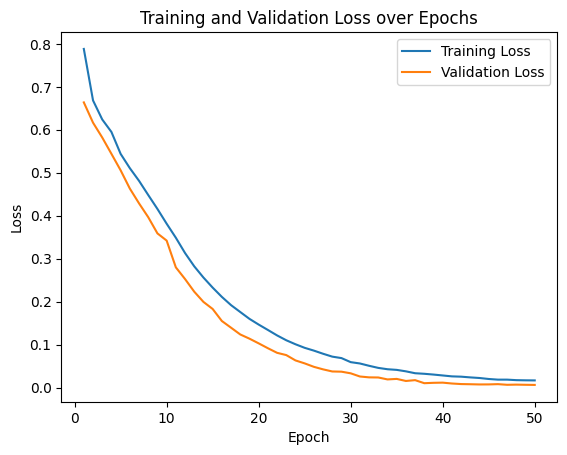
\includegraphics[width=0.8\linewidth]{img/lossgraph.png}
           \caption{Loss Curve}
           \label{fig:Loss curve over 50 epochs}
       \end{figure}
       \pagebreak
       \subsection{Word Error Rate(WER) and Character Error Rate(CER) Curve}
       At the beginning, we can observe WER and CER to be very high meaning the predictions are incorrect but as training goes on across increasing epochs, we see the value of these parameters decreasing meaning the model is learning to predict correctly with training. At the 50\textsuperscript{th} epoch both WER and CER is close to 0 meaning the predictions are close to actual words.
       \begin{figure}[h]
           \centering
           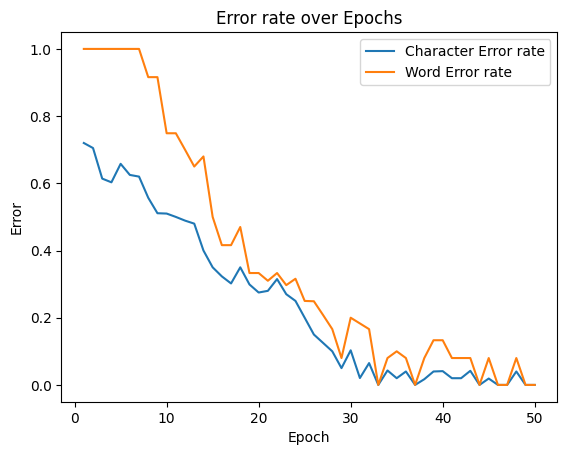
\includegraphics[width=0.8\linewidth]{img/wer.png}
           \caption{WER \& CER Curve}
           \label{fig:enter-label}
       \end{figure}
       \subsection{Testing Phase}
       The average values of \textbf{Word Error Rate(WER)} and \textbf{Character Error Rate(CER)} was calculated to be \textbf{0.1706} and \textbf{0.0712} over 50 test videos, all different from the ones used in training and validation. Meaning the model was able to predict 83\% of the words correctly and 93\% of the characters correctly. Even more accuracy on test videos can be achieved by training the model for more number of epochs.